\section{Chapter 1: WaveNet}
The WaveNet paper presents a CNN-based approach to generating audio samples. \cite{oord_wavenet_2016}
Instead of using RNNs as a recurrent architecture, the generative model only conditions on past samples, and as such does not include any hidden "state".

The probability of a waveform \(\mathbf{x}\in \mathbb{R}^T\) is expressed purely as:
\begin{equation}\label{eq:wavenet-probabilities}
    p(\mathbf{x}) = \prod_{t=1}^T  p(x_t | x_1, ..., x_t )
\end{equation}
where $ p(x_t | x_1, ..., x_t ) $ is parametrized only by the \textit{weights} in the network. 


\subsection{Architecture and design}
The WaveNet Architecture draws advantage from three developments: quantized output spaces (as shown in PixelRNN), dilated causal convolutions and gated activation units,

\paragraph{Quantized Output Space with $\mu$ law companding transformation}
Given an audio waveform \(\mathbf{x} \in [-1,1]^T\), transform the audio according to :
\begin{equation}
    f(x_t) = \textrm{sign}(x_t) \frac{ \ln(1 - \mu|x_t|  )}{ \ln(1 + \mu)  }
\end{equation} 
with \(\mu = 255\).


\paragraph{Dilated Causal Convolutions}
A \textit{Causal} Convolution is a fancy way of saying that audio convolutions only work forward in time, not backward.
This is to enforce the forward dependency in \cref{eq:wavenet-probabilities}.

A \textit{Dilated} Convolution is a convolution where the convolution kernel skips over a dimension, increasing the receptive field and observing more of the surrounding environment. 
For an image the simplest dilated convolutional is illustrated in \cref{fig:wavenet-dilated-conv}
\begin{figure}[!ht]
    \begin{small}
        \begin{center}
            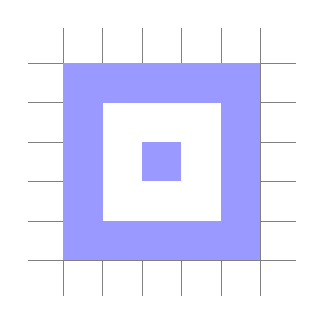
\begin{tikzpicture}
                \draw[step=0.5cm,gray,very thin] (-1.45,-1.45) grid (1.95,1.95);

                \fill[blue!40!white] (-1,-1) rectangle (1.5,1.5);
                \fill[white] (-0.5,-0.5) rectangle (1,1);
                \fill[blue!40!white] (0,0) rectangle (0.5,0.5);

            \end{tikzpicture}
        \end{center}
        \caption{A Simple Pixel Dilated Convolution}
        \label{fig:wavenet-dilated-conv}
    \end{small}
\end{figure}

Accordingly, for an audio signal, it would look like what we see in \cref{fig:wavenet-dilated-causal-conv}



\begin{figure}
    \begin{small}
        \begin{center}
            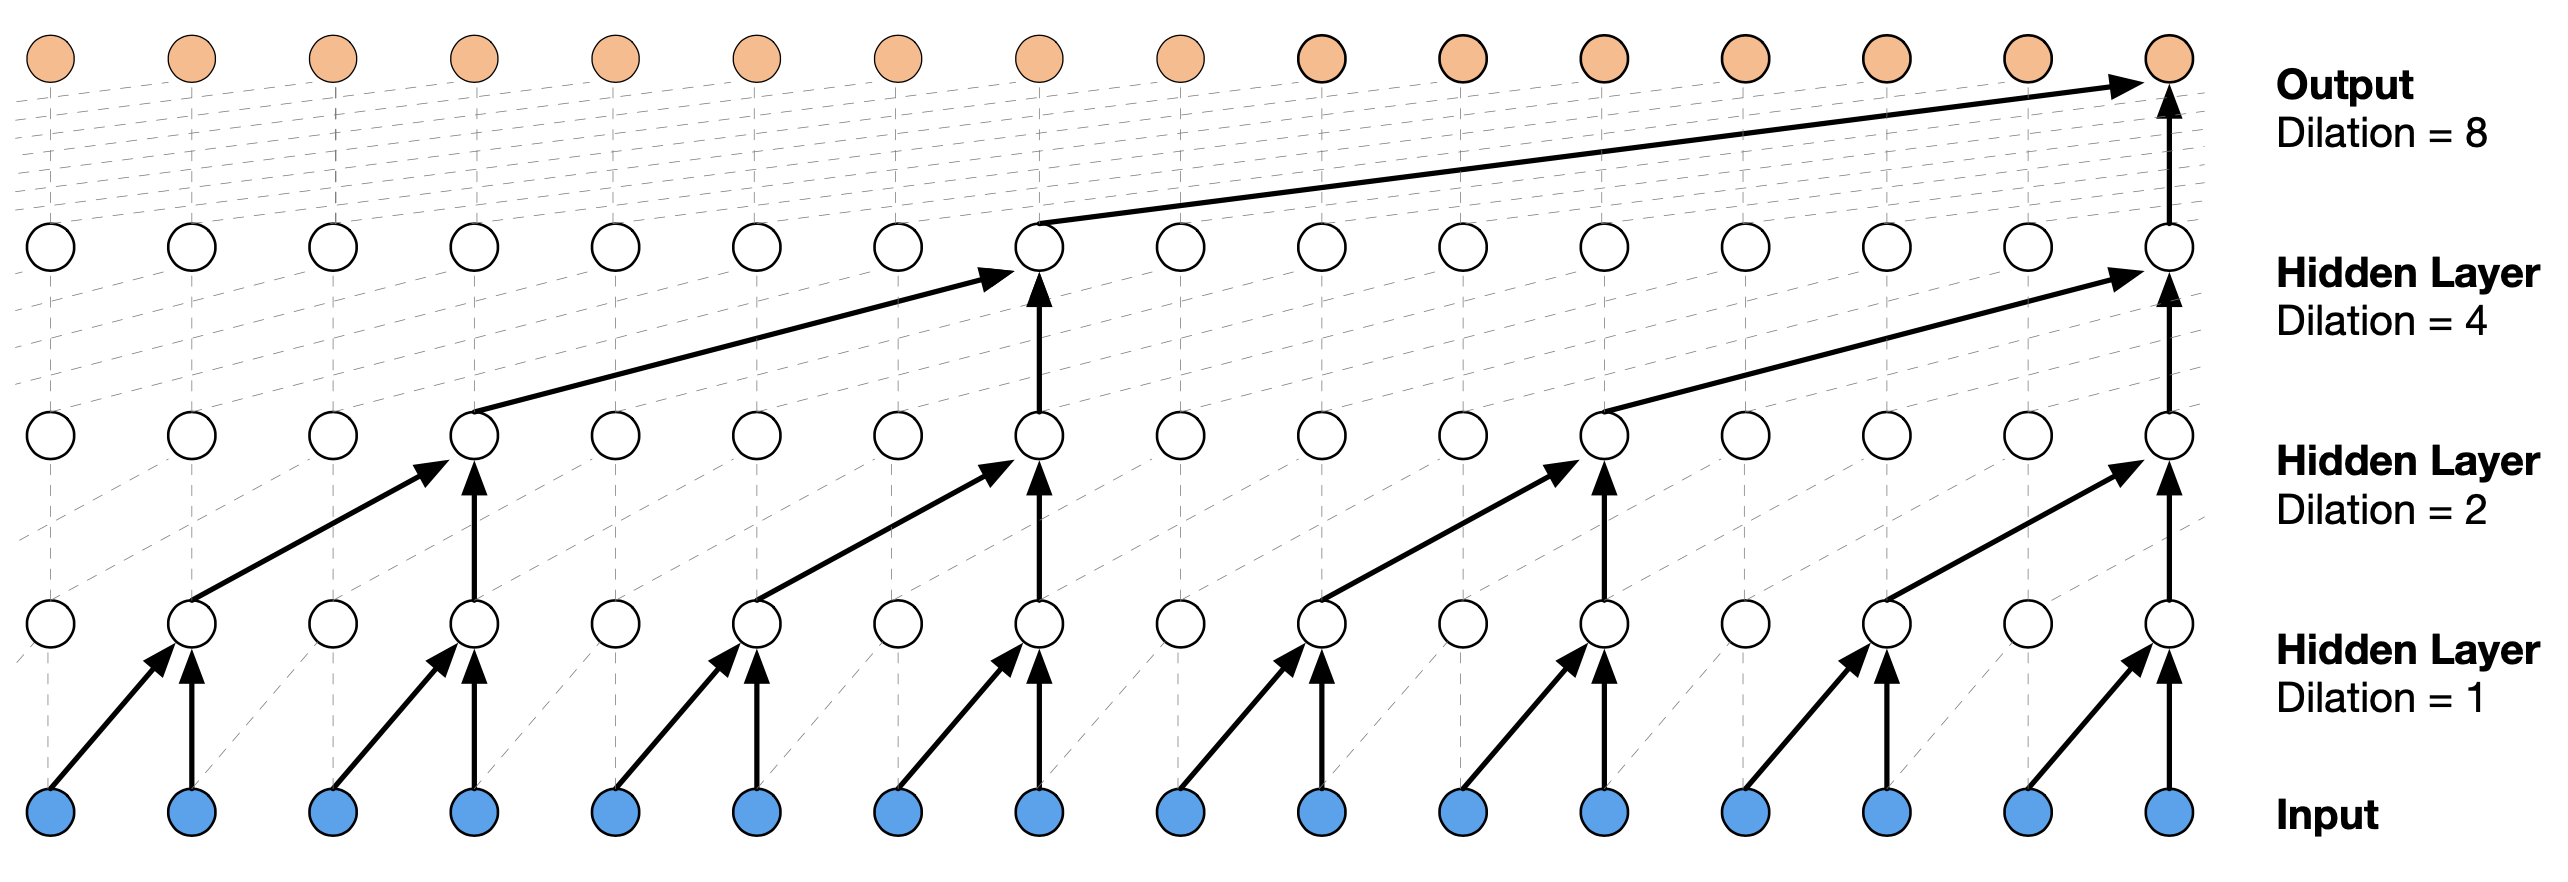
\includegraphics[width=0.95\textwidth]{figures/wavenet-dilated-causal-conv.png}
        \end{center}
        \caption{The Dilated Causal Convolution in WaveNet} 
        \label{fig:wavenet-dilated-causal-conv}
    \end{small}
\end{figure}



\paragraph{Gated Activation Units}
Each Convolution layer, Insteadof \textit{just} having a filter weight, also has a \textbf{gating weight}.
Hence the weights \(\mathbf{W} \in \mathbb{R}^{K \times 2} \), with \(K\) as the number of layers. 
The operation of layer $k \in [0, K]$, is parametrized as: 

\begin{equation}
    \mathbf{z} = \tanh ( \mathbf{x} * W_{k, f} ) \odot \sigma ( \mathbf{x} * W_{k, g} )
    \label{eq:wavenet-gated-activation}
\end{equation}





\paragraph{Summary of architechture}
The architecture is summed up in \cref{fig:wavenet-architecture}.
It's important to note that the Causal Convolution setup as described in \cref{fig:wavenet-dilated-causal-conv} only is applied \textit{once}, as the first layer.
This makes the entire rest of the network a simple convolutional network with dilation, as the \textbf{first (causal) convolutional stack ensures that the rest of the network will only see samples from the past.}
In all other respects we can consider this a standard CNN architecture. 


\begin{figure}
    \begin{small}
        \begin{center}
            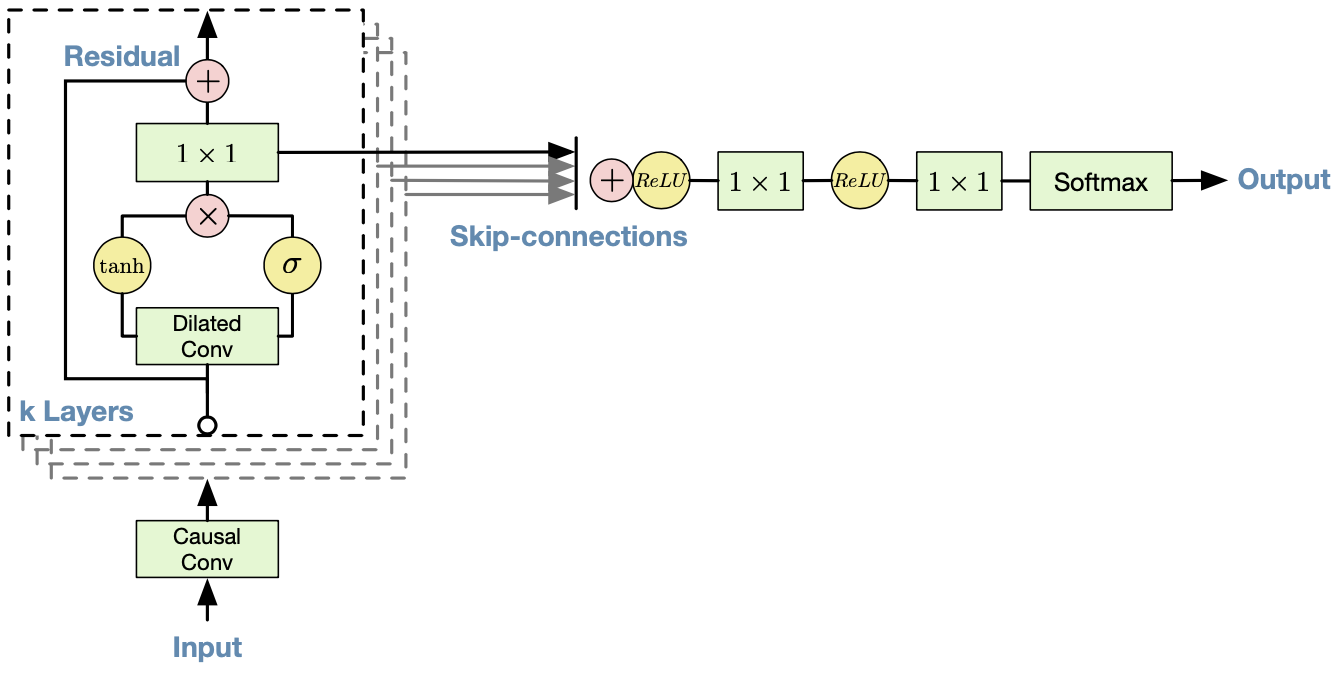
\includegraphics[width=0.95\textwidth]{figures/wavenet-architecture.png}
        \end{center}
        \caption{Overall Residual Architecture of WaveNet. 
        Skip connections happen from \textit{every Convolutional Layer} to the final softmax.}
        \label{fig:wavenet-architecture}
    \end{small}
\end{figure}


\subsubsection{Extending architecture to include latent representations of speaker}
It's possible to add a latent representation \(\mathbf{h}\), extending \cref{eq:wavenet-probabilities} to:

\begin{equation}\label{eq:wavenet-probabilities-ext}
    p(\mathbf{x}|\mathbf{h}) = \prod_{t=1}^T  p(x_t | x_1, ..., x_t, \mathbf{h} )
\end{equation}

There are two ways to represent this:

\paragraph{Global Conditioning (Speaker, Accent, Noise level)}
Here we set \(\mathbf{h}\) to a single global latent, representing a constant over the entire sequence. 
The activation from \cref{eq:wavenet-gated-activation} then becomes

\begin{equation}
    \mathbf{z} = \tanh ( \mathbf{x} * W_{k, f} + V^T_{k, f}\mathbf{h}) \odot \sigma ( \mathbf{x} * W_{k, g} + V^T_{k, g}\mathbf{h})
\end{equation}
With \(V_{k, *}\) is a linear projection , and the resulting vector \(V^T_{k, f}\mathbf{h}\) is broadcast over time \(T\).


\paragraph{Local Conditioning (Tone of voice, changing noise levels over the call}
Here we define \(h_t\), and use a ConvNet to upsample \(h_t\) to \(\mathbf{y} = f(\mathbf{h})\), so \cref{eq:wavenet-gated-activation} becomes:

\begin{equation}
    \mathbf{z} = \tanh ( \mathbf{x} * W_{k, f} + V_{k, f}*\mathbf{y}) \odot \sigma ( \mathbf{x} * W_{k, g} + V_{k, g}*\mathbf{y})
\end{equation}

\subsection{Results}

The main results here are evaluated on "subjective naturalness" by human evaluators. 
As such, WaveNets have outperformed previos TTS methods.
That's not really that interesting but it makes for a cool listen: \href{https://deepmind.com/blog/article/wavenet-generative-model-raw-audio}{here}